%%%%%%%%%%%%%%%%%%%%%%%%%%%%%%%%%%%%%%%%%%%%%%%%%%%%%%%%%%%%%%%%%%%%%%
%%
%% Thesis.tex -- Chenchong Charles Zhu graduate thesis.  Based on 
%% ut-thesis.tex
%%
%%     http://www.ctan.org/tex-archive/macros/latex/contrib/ut-thesis/
%%
%% with modifications (mostly based off Mubdi Rahman's thesis template):
%%  - ifpdf is used to control pdf figures
%%  - ifpdf is used to control pdf figures
%%
%%%%%%%%%%%%%%%%%%%%%%%%%%%%%%%%%%%%%%%%%%%%%%%%%%%%%%%%%%%%%%%%%%%%%%
%%
%% Copyright (c) 1998-2013 Francois Pitt <fpitt@cs.utoronto.ca>
%% last updated at 16:20 (EDT) on Wed 25 Sep 2013
%%
%% This work may be distributed and/or modified under the conditions of
%% the LaTeX Project Public License, either version 1.3c of this license
%% or (at your option) any later version.
%% The latest version of this license is in
%%     http://www.latex-project.org/lppl.txt
%% and version 1.3c or later is part of all distributions of LaTeX
%% version 2005/12/01 or later.
%%
%% This work has the LPPL maintenance status "maintained".
%%
%% The Current Maintainer of this work is
%% Francois Pitt <fpitt@cs.utoronto.ca>.
%%
%% This work consists of the files listed in the accompanying README.
%%
%% SUMMARY OF FEATURES:
%%
%% All environments, commands, and options provided by the `ut-thesis'
%% class will be described below, at the point where they should appear
%% in the document.  See the file `ut-thesis.cls' for more details.
%%
%% To explicitly set the pagestyle of any blank page inserted with
%% \cleardoublepage, use one of \clearemptydoublepage,
%% \clearplaindoublepage, \clearthesisdoublepage, or
%% \clearstandarddoublepage (to use the style currently in effect).
%%
%% For single-spaced quotes or quotations, use the `longquote' and
%% `longquotation' environments.
%%
%%%%%%%%%%%%%%%%%%%%%%%%%%%%%%%%%%%%%%%%%%%%%%%%%%%%%%%%%%%%%%%%%%%%%%

%%%%%%%%%%%%         PREAMBLE         %%%%%%%%%%%%

%%  - Default settings format a final copy (single-sided, normal
%%    margins, one-and-a-half-spaced with single-spaced notes).
%%  - For a rough copy (double-sided, normal margins, double-spaced,
%%    with the word "DRAFT" printed at each corner of every page), use
%%    the `draft' option.
%%  - The default global line spacing can be changed with one of the
%%    options `singlespaced', `onehalfspaced', or `doublespaced'.
%%  - Footnotes and marginal notes are all single-spaced by default, but
%%    can be made to have the same spacing as the rest of the document
%%    by using the option `standardspacednotes'.
%%  - The size of the margins can be changed with one of the options:
%%     . `narrowmargins' (1 1/4" left, 3/4" others),
%%     . `normalmargins' (1 1/4" left, 1" others),
%%     . `widemargins' (1 1/4" all),
%%     . `extrawidemargins' (1 1/2" all).
%%  - The pagestyle of "cleared" pages (empty pages inserted in
%%    two-sided documents to put the next page on the right-hand side)
%%    can be set with one of the options `cleardoublepagestyleempty',
%%    `cleardoublepagestyleplain', or `cleardoublepagestylestandard'.
%%  - Any other standard option for the `report' document class can be
%%    used to override the default or draft settings (such as `10pt',
%%    `11pt', `12pt'), and standard LaTeX packages can be used to
%%    further customize the layout and/or formatting of the document.

%% *** Add any desired options. ***
\documentclass{ut-thesis}

%% *** Add \usepackage declarations here. ***
%% The standard packages `geometry' and `setspace' are already loaded by
%% `ut-thesis' -- see their documentation for details of the features
%% they provide.  In particular, you may use the \geometry command here
%% to adjust the margins if none of the ut-thesis options are suitable
%% (see the `geometry' package for details).  You may also use the
%% \setstretch command to set the line spacing to a value other than
%% single, one-and-a-half, or double spaced (see the `setspace' package
%% for details).

% ifpdf conditional
\usepackage{ifpdf}

\ifpdf
\usepackage[pdftex]{graphicx}
\usepackage[protrusion=true,expansion=true]{microtype}
\else
\usepackage{graphicx}
\fi

% symbols & math
%\usepackage{latexsym}
%\usepackage{amssymb}

% hyperlinks within document
\usepackage{hyperref}

% bibliography
\usepackage{natbib}
\setcitestyle{aysep={},yysep={;}}

% include AASTeX
\usepackage{aastex_commands}
%\usepackage{deluxetable}
%\usepackage[labelsep=colon,small]{caption}

% fonts
\usepackage[sc]{mathpazo}
\usepackage[T1]{fontenc}

%%%%%%%%%%%%%%%%%%%%%%%%%%%%%%%%%%%%%%%%%%%%%%%%%%%%%%%%%%%%%%%%%%%%%%%%
%%                                                                    %%
%%                   ***   I M P O R T A N T   ***                    %%
%%                                                                    %%
%%  Fill in the following fields with the required information:       %%
%%   - \degree{...}       name of the degree obtained                 %%
%%   - \department{...}   name of the graduate department             %%
%%   - \gradyear{...}     year of graduation                          %%
%%   - \author{...}       name of the author                          %%
%%   - \title{...}        title of the thesis                         %%
%%%%%%%%%%%%%%%%%%%%%%%%%%%%%%%%%%%%%%%%%%%%%%%%%%%%%%%%%%%%%%%%%%%%%%%%

%% *** Change this example to appropriate values. ***
\degree{Doctor of Philosophy}
\department{Astronomy \& Astrophysics}
\gradyear{2016}
\author{Chenchong Zhu}
\title{Shedding Light on Carbon-Oxygen White Dwarf Mergers and Post-Merger Evolution}

%% *** NOTE ***
%% Put here all other formatting commands that belong in the preamble.
%% In particular, you should put all of your \newcommand's,
%% \newenvironment's, \newtheorem's, etc. (in other words, all the
%% global definitions that you will need throughout your thesis) in a
%% separate file and use "\input{filename}" to input it here.

\newcommand{\domm}[1]{\ifmmode #1\else$#1$\fi}

\newcommand{\azero}{\domm{a_0}}
\newcommand{\Msun}{\domm{M_{\odot}}}
\newcommand{\Rsun}{\domm{R_{\odot}}}
\newcommand{\Mch}{\domm{M_{\rm Ch}}}
\newcommand{\Ni}{\hbox{$^{56}$Ni}}
\newcommand{\pyr}{\domm{{\rm yr}^{-1}}}
\newcommand{\psec}{\domm{{\rm s}^{-1}}}
\newcommand{\gcc}{\domm{{\rm g\,cm}^{-3}}}


%% *** Adjust the following settings as desired. ***

%% List only down to subsections in the table of contents;
%% 0=chapter, 1=section, 2=subsection, 3=subsubsection, etc.
\setcounter{tocdepth}{2}

%% Make each page fill up the entire page.
\flushbottom


%%%%%%%%%%%%      MAIN  DOCUMENT      %%%%%%%%%%%%

\begin{document}

%% This sets the page style and numbering for preliminary sections.
\begin{preliminary}

%% This generates the title page from the information given above.
\maketitle

%% There should be NOTHING between the title page and abstract.
%% However, if your document is two-sided and you want the abstract
%% _not_ to appear on the back of the title page, then uncomment the
%% following line.
%\cleardoublepage

%% This generates the abstract page, with the line spacing adjusted
%% according to SGS guidelines.
\begin{abstract}
%% *** Put your Abstract here. ***
%% (At most 150 words for M.Sc. or 350 words for Ph.D.)
\end{abstract}

%% Anything placed between the abstract and table of contents will
%% appear on a separate page since the abstract ends with \newpage and
%% the table of contents starts with \clearpage.  Use \cleardoublepage
%% for anything that you want to appear on a right-hand page.

%% This generates a "dedication" section, if needed -- just a paragraph
%% formatted flush right (uncomment to have it appear in the document).
%\begin{dedication}
%% *** Put your Dedication here. ***
%\end{dedication}

% Here's Mubdi's version
\vspace*{\fill}
\begin{center}
\begin{minipage}[c]{4.75in}
  ``Do or do not; there is no try.''\vspace{2em}

\hfill \emph{--Yoda}

\end{minipage}
\end{center}
\vspace*{\fill}

%% The `dedication' and `acknowledgements' sections do not create new
%% pages so if you want the two sections to appear on separate pages,
%% uncomment the following line.
%\newpage  % separate pages for dedication and acknowledgements

\cleardoublepage

%% Alternatively, if you leave both on the same page, it is probably a
%% good idea to add a bit of extra vertical space in between the two --
%% for example, as follows (adjust as desired).
%\vspace{.5in}  % vertical space between dedication and acknowledgements

%% This generates an "acknowledgements" section, if needed
%% (uncomment to have it appear in the document).
\begin{acknowledgements}
I'd like to thank the academy for choosing me...
\end{acknowledgements}

%% This generates the Table of Contents (on a separate page).
\tableofcontents

%% This generates the List of Tables (on a separate page), if needed
%% (uncomment to have it appear in the document).
\listoftables

%% This generates the List of Figures (on a separate page), if needed
%% (uncomment to have it appear in the document).
\listoffigures

%% You can add commands here to generate any other material that belongs
%% in the head matter (for example, List of Plates, Index of Symbols, or
%% List of Appendices).

%% End of the preliminary sections: reset page style and numbering.
\end{preliminary}


%%%%%%%%%%%%%%%%%%%%%%%%%%%%%%%%%%%%%%%%%%%%%%%%%%%%%%%%%%%%%%%%%%%%%%%%
%%  Put your Chapters here; the easiest way to do this is to keep     %%
%%  each chapter in a separate file and `\include' all the files.     %%
%%  Each chapter file should start with "\chapter{ChapterName}".      %%
%%  Note that using `\include' instead of `\input' will make each     %%
%%  chapter start on a new page, and allow you to format only parts   %%
%%  of your thesis at a time by using `\includeonly'.                 %%
%%%%%%%%%%%%%%%%%%%%%%%%%%%%%%%%%%%%%%%%%%%%%%%%%%%%%%%%%%%%%%%%%%%%%%%%

%% *** Include chapter files here. ***

\chapter{Introduction}

%%The merger of two white dwarfs (WDs) originally in a short-period binary is estimated (eg. \citealt{badem12}) to occur about once every century in a Milky Way-like galaxy, making the products of such events common throughout the universe.  They have been held responsible for producing a variety of stars with strange properties, including helium-burning sdOB stars \citep{saioj00, justph11}, RCrB stars (eg. \citealt{webb84, clay+07, clay13}), and massive and highly magnetized WDs (eg. \citealt{segrcm97, garc+12, kule+13}) that could resemble the hot DQ WDs (eg. \citealt{dunlc15}, Dunlap and Clements in preparation).  They may, however, also be responsible for spectacular transient events including accretion-induced collapses (eg. \citealt{saion85, abdi+10}) and type Ia supernovae (SNe Ia; eg. \citealt{howe11, hill+13, maozmn14}).  Determining the final outcome of a particular merger requires an understanding of the detailed dynamics of the merging process, which cannot directly be seen using current observational capabilities.  Thus, studies of merger physics have primarily utilized hydrodynamic simulations.

Approximately two out of every three stars are born into a binary system.  A substantial fraction of these stars will interact, some following the expansion of one or both constituent stars as they evolve off of the main sequence, and others after gravitational radiation, magnetic braking or three-body dynamics drastically shrink their orbital separation.  These interactions primarily take the form of mass transfer between the stars, and if mass transfer becomes unstable, it ends with the violent coalescence of the two stars into one.  These stellar mergers, like other forms of binary interaction, disrupt single star evolution and create merged products, or ``merger remnants'', with unusual properties.

Mergers also liberate energy on the order of the gravitational binding energy of the binary and can eject copious amounts of mass, giving rise to a cornucopia of electromagnetic (and gravitational-wave) transients ranging from luminous red novae (from the merger of two (post-) main-sequence stars; eg. V838 Monocerotis and V1309 Scorpii \citep{tyle+11, nandil14}) to short gamma-ray bursts (from two neutron stars or a neutron star and a black hole; eg. \citealt{ross15}) and the gravitational wave outburst from coalescing stellar-mass black holes (as recently found by the Advanced Laser Interferometer Gravitational-Wave Observatory (LIGO); \citealt{ligo16}).  Indeed, with current deep and short-cadence optical/near-infrared survey projects such as the Palomar Transient Factory \citep{rau+09} and Pan-STARRS \citep{kais+10} continuing to uncover more uncommon and even hitherto-unknown transients, and the ambitious Large Synoptic Survey Telescope \citep{lsst09} under construction, a much more complete picture of merger-generated transients will form over the next decade.

In this thesis, I will be examining the merger and post-merger evolution of two carbon-oxygen white dwarfs to determine the sorts of merged products and transients they create.  In particular, I investigate if they can produce thermonuclear, or type Ia, supernovae, even if their total mass is below the Chandrasekhar mass.  I will first discuss the mergers of white dwarfs in general, and the diverse array of unusual stars and explosions they could potentially generate.  I will then focus on the possible outcomes for mergers of sub-Chandrasekhar carbon-oxygen white dwarf binaries, and elaborate on why novel mechanisms for making type Ia supernovae are needed.

% Sec 5.2.3 of Tylenda talks about MS - MS pre-merger orbital evolution.

\section{Mergers of Two White Dwarfs}
\label{sec:c1_wdmergers}

Stars with masses $\lesssim8\,\Msun$ generally end their lives as white dwarfs (WDs).  On their own, WDs are inert: held up against gravity by electron degeneracy pressure and having ceased nuclear fusion, they will slowly radiate away their remaining thermal energy over billions of years.  WDs in interacting binaries, on the other hand, can receive mass and energy from their stellar companion, leading to a whole host of energetic and potentially explosive phenomena.

%\subsection{The Formation of Double White Dwarf Binaries}
%\label{ssec:c1_ddwdform}

Among double WD binaries, a fair number are in extremely close orbits, with periods ranging from hours to minutes.  As these periods correspond to orbital separations well within the radii of red and asymptotic giant branch stars, the WD pairs are formed from systems that have experienced at least two episodes of mass transfer (eg. \citealt{nele+01a, toonnp12, toon+14}).  These can sap the orbital angular momentum of the binary through mass loss, and so close double WDs tend to come from systems where (at least) the final mass transfer phase is a ``common envelope event'' where one star enters the envelope of the other and much of this envelope is ejected.\footnote{Binaries may also experience a ``double common envelope event'' -- where both stars simultaneously envelop one another -- and other unusual interactions.  See eg. \cite{toonnp12} and the Appendix of \cite{toon+14} for overviews of the formation channels of close double WD binaries.}

%http://adsabs.harvard.edu/abs/2008MNRAS.387.1693C
%The mass parameter space of double WD binaries, subdivided by their chemical composition,
\begin{figure}
\centering
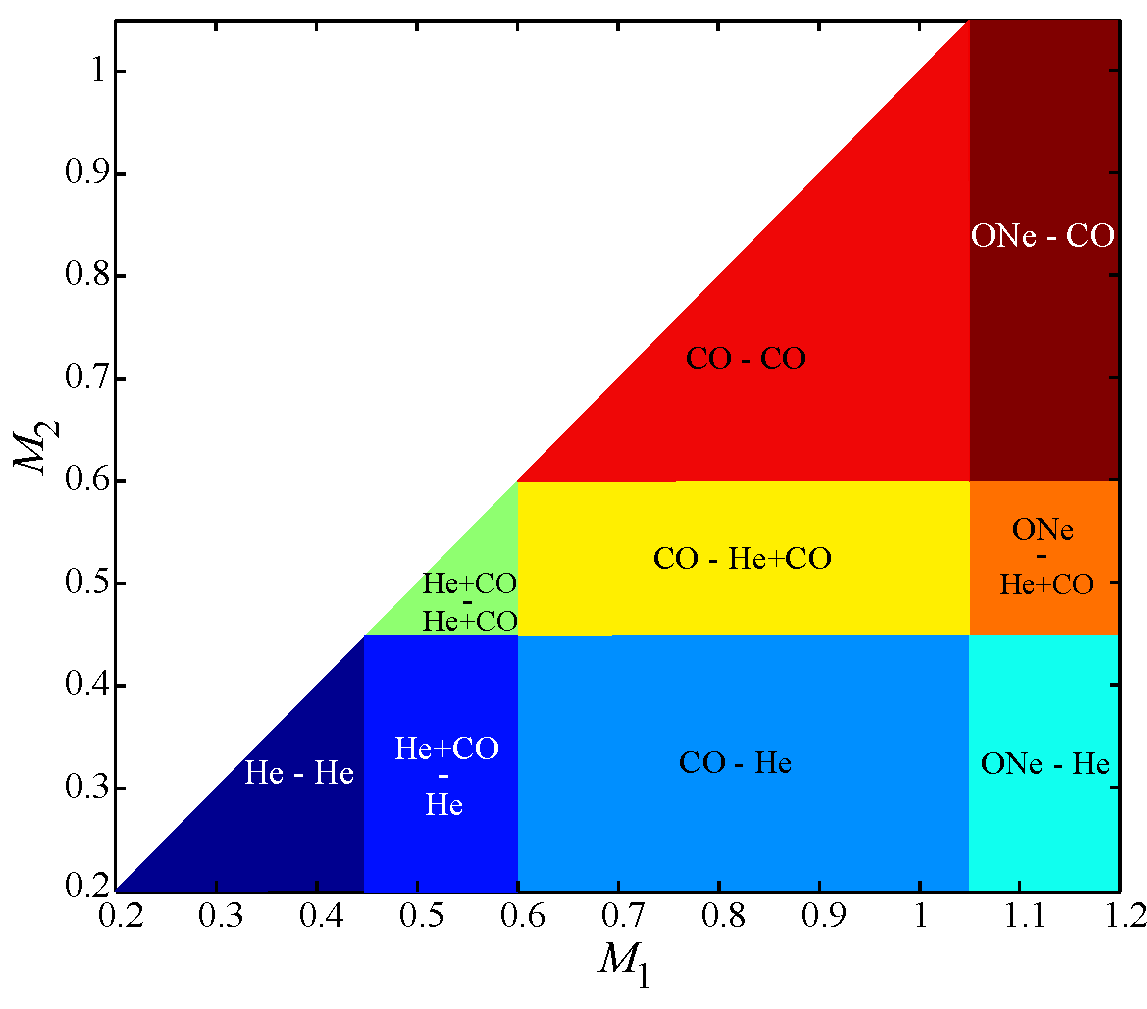
\includegraphics[width=0.6\hsize]{introduction/figures/dan+12_wdbinmass.pdf}
\caption{The expected compositions for white dwarfs undergoing a merger as a function of their masses, from \citeauthor{dan+12} (\citeyear{dan+12}, their Fig. 1).  $M_1$ is the mass of the accretor, or primary, WD (\Ma\ in the text), and $M_2$ is the mass of the donor, or secondary (\Md).  WDs with masses $M<0.45\,\Msun$ are assumed to be He WDs, those with $0.45 < M < 0.6\,\Msun$ CO WDs with thick He envelopes, $0.6 < M < 1.05\,\Msun$ CO WDs, and $M>1.05\,\Msun$ ONe WDs.  See text, as well as \cite{dan+12} Sec. 2, for discussion on these choices.}
\label{fig:c1_wdbinarymasses}
\end{figure}

% He flash - eg. \citealt{kippww12}, Ch. 33.4
% He WDs need friends: eg. \citealt{kippww12}, Ch. 33.4

The mass and composition of each WD within the binary is dependent on the binary's prior evolution.  Broadly speaking, WDs with masses $M \lesssim 0.45\,\Msun$ are composed of helium (He); these come from stars that had their evolution interrupted by binary interaction while on the red giant branch (eg. \citealt{marsdd95, nele+01, nele+01a}), before their degenerate He core became massive enough to trigger a helium flash.\footnote{He and CO WDs with $M\lesssim0.5\,\Msun$ could in principle come from single stellar evolution, but these take longer than a Hubble time to evolve.}  WDs with slightly higher masses have extensive He envelopes of $\sim0.1\,\Msun$ surrounding cores composed of carbon and oxygen (CO; \citealt{ibent85}).  \cite{dan+12} approximate the mass range of these ``hybrid WDs'' to be $0.45 \lesssim M \lesssim 0.6\,\Msun$, and set the composition of the upper $0.1\,\Msun$ of these WDs to He in their simulations.  From $0.6 \lesssim M \lesssim 1.1\,\Msun$ WDs are almost entirely composed of CO, with He atmospheres of $\sim10^{-2}\,\Msun$ \citep{ibent85}.  WDs with masses $\gtrsim 1.1\,\Msun$ come from super-AGB stars (eg. \citealt{herw05}) that ignite carbon during their evolution (eg. \citealt{garc13}), and thus are composed at least partly of oxygen and neon (ONe).  

Fig. \ref{fig:c1_wdbinarymasses}, from \cite{dan+12}, summarizes these relationships -- in it, $M_1$ is the mass of the more massive primary WD, which accretes mass during the merger, and $M_2$ is the mass of the secondary, which donates mass (see Sec. \ref{ssec:c1_stable_mass_transfer} for why this is always the case).  In this thesis, we refer to these as \Ma\ and \Md, respectively.  While sophisticated stellar evolution calculations are not always so clear-cut (eg. \citealt{ibent85, moros09} for CO WDs with $M\lesssim0.45\,\Msun$ and \citealt{hurlpt00} for CO WDs with $M\gtrsim1.2\,\Msun$), these relationships are used as rules of thumb for setting WD composition for a wide range of works (\citealt{loreig09,rask+12,dan+12,dan+14}, with slight variations between them).  In this thesis, we look at binaries of pure CO WDs (without He atmospheres) with masses ranging from $0.4 - 1.0\,\Msun$.

% for our parameter space study of mergers in Ch. \ref{ch:ch2}.  

%In subsequent chapters, we are primarily interested in the the merger of two CO WDs near the median mass of field WDs, $\sim0.65\,\Msun$ (Sec. \ref{ssec:c1_cowd_massrange}).

%The ratio of carbon and oxygen within CO WDs is also not particularly well-known.  In this thesis, we make the assumption that they are composed of 50\% carbon and 50\% oxygen by mass.  {\charles ADD STUFF}

%\subsection{Orbital Angular Momentum Loss and Gravitational Wave Emission}
%\label{ssec:c1_inspiral}

%magnetic braking ({\charles important for AM Canum Venaticorum systems} eg. \citealt{verb84, knigbp11})

Following their formation, WD binaries lose orbital angular momentum by emitting gravitational radiation (eg. \citealt{petem63}).\footnote{They may also lose angular momentum through the influence of a third body (eg. \citealt{katzd12}); see Sec. \ref{ssec:c1_new_typeia}.}  This loss has a characteristic inspiral timescale of \citep{segrcm97}

\begin{eqnarray}
\tau_{\mrm{grav}} = \frac{L_\mrm{orb}}{|\dot{L}_\mrm{orb}|} &=& \frac{5c^5}{32G^3}\frac{a^4}{\Ma\Md\Mtot}\nonumber \\
&=&5 \times 10^5 \left(\frac{a}{10^5 \mrm{km}}\right)^4 \frac{\Msun}{\Ma} \frac{\Msun}{\Md} \frac{\Msun}{\Mtot}\,\mrm{yr}.
\label{eq:c1_gravtimescale}
\end{eqnarray}

\noindent where $L_\mrm{orb}$ is the orbital angular momentum and $a$ is the orbital separation.  From this, we see that WD binaries with orbital periods on the order of hours or less ($a \lesssim 10^6\,\mrm{km} \sim 0.01\,\mrm{AU}$) will merge within a Hubble time.  

%It is estimated that there are on order of $10^8$ such systems in the Milky Way alone \citep{mars11, nele+01a}. <- This may be somewhat true, but don't write this unless you can guarantee all of these will merge within a hubble time!

As an aside, the gravitational waves emitted by inspiralling WD binaries are detectable from Earth.  With periods on the order of minutes, they are too low-frequency to be detected by Advanced LIGO \citep{ligo+15}, but are expected to be the most numerous and dominant source of gravitational waves \citep{mars11} detected by the proposed spaceborne detector eLISA (evolved Laser Interferometer Space Antenna; \citealt{amar+13}), which probes the mHz - Hz frequency range.  The instrument will likely resolve individual signals from thousands of binaries with orbital periods on the order $\sim10$ minutes (and are thus close to merging; \citealt{amar+13, mars11, dan+11}), while numerous sources that are too far away or at longer orbital periods will comprised an unresolved background \citep{neleyp01,amar+13}.  Measurement of either of these will probe the WD binary population of the Milky Way without the selection biases that often trouble electromagnetic binary searches \citep{mars11}.  Note that gravitational radiation plays a negligible role in the actual merger, as the waves released during the merger have a total energy $\sim10^{-10}$ of the binary's binding energy (eg. \citealt{loreig09}).

%Note, however, that final coalescence of the WDs is over far too quickly to be detectable by eLISA.

\section{Merger Outcomes}
\label{sec:c1_mergeroutcomes}

Like any merger, those between WDs liberate of order their gravitational binding energy.  This can lead to enough heating and/or compression to reignite the nuclear furnaces of normally inert WDs.  As this may happen under either non-degenerate or degenerate circumstances, the end product of such mergers are diverse, ranging from stars with unusual properties undergoing stable nuclear burning to explosions. Additionally, hydrostatic WDs have a maximum stable mass beyond which they are unstable to collapse -- the \cite{chan31} mass, or \Mch, at $\sim1.4\,\Msun$.  This has long led to the notion that sufficiently massive WD mergers can result in the complete destruction of the merger product in a thermonuclear explosion that would resemble a type Ia supernova (SN Ia; \citealt{webb84}), or in its transformation into a neutron star (NS) in an event known as an accretion-induced collapse \citep{nomoi85, saion85}.  We now know of a much greater range of possible merger outcomes for both systems with masses above and below \Mch.  Which outcome occurs depends on the compositions of the WDs involved, and are briefly summarized below (see also \citealt{dan+14}, who produce a similar list):

% dan+14 Fig 12, dan+12 fig 8

\begin{itemize}
	\item The merger of {\bf two He WDs} is unlikely to lead to violent nuclear burning and an explosion \citep{dan+12,dan+14,dan+15}.  Instead, merger remnants with total masses $0.4\lesssim \Mtot \lesssim 0.8$ \citep{han+02,ibent85}\footnote{This is lower than the He flash mass of $\sim0.45\,\Msun$ because the merger remnant is partly non-degenerate \citep{ibent85, han+02}.}, which are the vast majority of double He WD remnants \citep{nele10}, are expected to ignite He burning in a shell.  \citep{saioj00} and \cite{zhanj12} calculate that He shell burning increases the radius and luminosity of the star, turning it over $\sim 10^3-10^4\,\mrm{yr}$ into a yellow giant.  Over the next $10^5-10^6\mrm{yr}$, the burning shell migrates inward with a series of weakening shell flashes, while the radius slowly shrinks to $\sim10^{-1}\,\Rsun$.  Once the shell reaches the center of the remnant, it settles onto the helium main sequence, and resembles a He-rich subdwarf B (sdB) or O (sdO) star \citep{saioj00, justph11, zhanj12, hebe16}.  Most subdwarf stars are in binaries -- and likely arise from other formation channels -- and there are multiple proposed mechanisms to produce single sdB stars (such as a merger between a low-mass star or brown dwarf and a red giant; \citealt{soke98}), and so the contribution of mergers to the sdB population remains unclear \citep{nele10, hebe16}.

%"with properties similar to Extreme Helium (EHe) and R Coronae Borealis (R CrB) stars \citep{saioj00, zhanj12}", but this then makes the description too confusing.

% See conclusion section of hebe16 for alternate sources of single subdwarfs.  From hebe16: single sdBs tend to be narrowly peaked in mass, not obvious if mergers can do this.  Low mass MS star or brown dwarf may merge with RGB core to make single sdB in CE, He WD/MS merger.  From nele10: enhanced single star mass loss might do it too, but not obvious if this happens

%(\citealt{justph11}; He-poor sdO stars are likely evolved sdB stars)

	\item The outcome of a merger between {\bf an He and a CO WD}, or a merger between an He and hybrid He-CO WD, depends on whether or not a He explosion is touched off during the merger.  Roughly speaking, mergers with $\Mtot \lesssim 0.8\,\Msun$ will lead to steady He burning in a shell, and are thought to be the progenitors to He-rich sdO stars \citep{justph11}.  Mergers with $\Mtot \gtrsim 0.8\,\Msun$ that do not experience an explosion will also ignite shell burning, but unlike sdOB progenitors they will retain their extended envelope over the lifetime of the He-burning shell \citep{ibent85, zhanj12b}.  These mergers are believed to be the primary formation channel for Hydrogen-deficient Carbon (HdC) and R CrB stars (eg. \citealt{webb84, ibent84, saioj02, clay12, zhan+14}), which are H-deficient, He- and C-rich supergiants that, in the case of R CrB stars, feature abrupt variability by up to a factor of $\sim10^3$ due to the formation of carbon dust above their photospheres.\footnote{Subdwarf stars formed from double He WD mergers with $\Mtot \gtrsim 0.8\,\Msun$ will also expand to become R CrB stars following core He exhaustion, but this formation channel accounts for only a few percent of all R CrBs \citep{zhanj12b}.}  Following He shell exhaustion, they will contract in radius and heat their envelopes, resembling EHe stars \cite{saioj02, jeff14}.

Helium explosions become more likely for binaries with $\Mtot\gtrsim\Mch$ \citep{dan+12, dan+14}.  In cases where an accreted He shell explodes, but the underlying CO WD remains, the result depends on a number of factors including the mass of the CO WD and amount of He it accretes, and spans a wide range of possible peak luminosities \citep{woosk11}.  Detonations (or deflagrations; \citealt{woosk11}) of $\lesssim0.1\,\Msun$ He shells lead to explosions that reach peak brightnesses $\sim10-100$ fainter than SNe Ia over $\sim2-10$ days (typical SNe Ia values are in Sec. \ref{sec:c1_mysteryofsneia}), making them similar to the ``.Ia SNe'' theorized to occur in AM Canum Venaticorum binaries \citep{bild+07}.  They synthesize Ca, Cr and Ti, but relatively little of the radioactive \Ni\ typically seen in SNe Ia \citep{shen+10he, woosk11, wald+11}.  Denser He envelopes (due to it or the CO WD accretor being more massive), tend to synthesize more \Ni\ in detonations \citep{shen+10he, wald+11}. 

%As an aside, \cite{wald+11} also suggest that the detonation of $\sim0.2\,\Msun$ of He on top of a $\sim0.45\,\Msun$ CO WD could explain the SN 2005E-like class of low-luminosity SNe Ib that produce very little \Ni, have low ejecta masses and spectroscopically show strong lines of He, Ca and Ti \citep{pere+10}.  Their initial conditions (and those of \cite{shen+10he}) assume the He envelopes were constructed through slow ($\lesssim10^{-6}\,\Msun\,\pyr$) accretion onto the CO cores until He nuclear runaway is triggered through compressional heating.  Mergers between low-mass CO and He WDs will likely generate He envelopes that are far less degenerate, and which will not experience such a nuclear runaway.

% moreover simulations suggest He detonations in mergers occur before an He envelope of more than a few $10^{-2}\,\Msun$ can accrete onto the disk.

%Less degenerate material will lead to explosions dominated by lighter elements like Ca \citep{woosk11}, and therefore He detonation may be possible in really massive systems.  Dan+14 already had that idea though; see below.

In the case where the the He shell detonates, and triggers the CO WD to do the same, a ``double-detonation'' SN Ia may be produced (Sec. \ref{ssec:c1_new_typeia}).

	\item The merger of {\bf two CO WDs} has long been suspected of producing an SN Ia under the right conditions (Sec. \ref{sec:c1_mysteryofsneia} and \ref{sec:c1_vkchannel}).  If these conditions are not met, they will instead create a lone massive, rotating and highly magnetized CO WD or, if steady carbon fusion is ignited, a carbon-burning star that eventually turns into an ONe WD (Sec. \ref{sec:c1_hotdqs}).  If the ONe WD is above \Mch, it may collapse into a neutron star (see below).

	\item Due to their mass, it is likely that the merger of {\bf an ONe WD} with any companion will create a super-\Mch\ remnant.  Unlike their CO counterparts, an ONe WD that is compressed through accretion to $\gtrsim3\times10^9\,\gcc$ initiates electron-capture reactions onto $^{20}$Ne and $^{24}$Mg, losing degeneracy support in the process (eg. \citealt{miya+80, saion85, schwqb15}).  This leads to further contraction, which likely ends\footnote{Since the electron capture reactions are exothermic, they trigger a thermal runaway that eventually starts an O-deflagration at $\sim10^{10}\,\gcc$.  Whether or not collapse or explosion occurs depends on exactly when the deflagration ignites; see eg. discussion in \cite{schwqb15}.} in an ``accretion-induced collapse'' (AIC) into a neutron star soon after its central density reaches $\sim10^{10}\,\gcc$ \citep{schwqb15}.  Simulations \citep{dess+06, dess+07, frye+09} of the AIC find it expels only $\sim10^{-2}\,\Msun$ of ejecta and produces negligible amounts of radioactive \Ni, suggesting a very faint transient.

%Note - oxygen pycnonuclear fusion occurs well beyond 10^10 gcc (Fig. 12 Schw+15)

\cite{dan+14} discusses the possibility that He - ONe and CO - ONe WD mergers will lead to enshrouded AIC that produce ``hybrid supernovae'', where much of the outer envelope (of a different composition) explodes rather than collapsing.  In particular, they suggest (based on the \cite{shen+10he} and \cite{wald+11} simulations above) that the detonation of the thick He envelope of a significantly super-\Mch\ He - ONe WD merger remnant could  explain the SN 2005E-like class of low-luminosity SNe Ib that produce very little \Ni, have low ejecta masses and spectroscopically show strong lines of He, Ca and Ti \citep{pere+10}.

\cite{marq+15} suggest that an ONe WD could be detonated through binary interactions in the same manner as CO WDs (Sec. \ref{ssec:c1_new_typeia}).  Due to their high densities, these would produce $\gtrsim1\,\Msun$ of \Ni, but, because fusing to \Ni\ from O and Ne generates $\sim30$\% less energy than from C \citep{marq+15}, they would also be weaker than CO WD detonations.  Detonations during ONe mergers may explain supernovae such as SN 2009dc \citep{taub+09} that have a peak brightness $\sim3$ times higher, and decay from peak brightness $\sim3$ times more slowly, than SNe Ia, and also have low expansion velocities.

\end{itemize}

Of these possibilities, ones that create SNe Ia are particularly intriguing, as they may hold the key to solving the long-standing problem of how these explosions arise.

\chapter{Chapter 2}

\chapter{Chapter 3}

\chapter{Conclusion}

What, then, has our body of work, as well as the numerous other recent investigations into mergers and post-merger evolution, taught us about the fate of sub-\Mch\ CO WD mergers?  Are there systems that compress and heat enough during post-merger evolution to ignite degenerate carbon burning near their centers, which then leads to an explosion?  Below, I summarize our current understanding of these systems and the sub-\Mch\ merger channel scenario proposed by \citeal{vkercj10}, and suggest avenues for future exploration.

\section{Mergers and Early Post-Merger Evolution}
\label{sec:c6_mergers_pme}

In Ch. \ref{ch:ch2}, we used SPH simulations of double CO WD mergers to explore the range of possible merger remnants and determine which among them are candidates for ignition under highly degenerate conditions during post-merger evolution.  The properties most important for this are the temperature and degree of rotational support of the dense remnant core, and we find that dissimilar-mass mergers result in cold and slowly-rotating cores that are unlikely to subsequently ignite, while similar-mass ones have cores that are heated abnd partly rotationally supported throughout.  The (rough) dividing line between the two classes is a density ratio between donor and accretor WD of $\qrho\simeq0.6$, equivalently a difference between their masses of $\Delta M \simeq 0.1\,\Msun$.

Since the publication of Ch. \ref{ch:ch2}, \cite{dan+14} published their study of remnants from synchronized WD mergers with exact initial conditions.  They find that for all of their merger remnants -- even ones we deem similar-mass -- the mass enclosed within the radius of maximum temperature \MencTmax\ is approximately the mass of the accreting WD, and the temperature at the remnant's center is a factor of at least a few lower.  Their similar-mass mergers also do not substantially mix, as ours do.  \cite{dan+14} link these differences to their use of synchronized and exact initial conditions, consistent with our findings in Sec. \ref{sec:c2_variation} that synchronization and longer periods of mass-transfer prior to coalescence make merger remnants resemble dissimilar-mass ones.

In Ch. \ref{ch:ch3} we compared a similar-mass $0.625-0.65\,\Msun$ merger simulated using SPH with one using the moving mesh code \arepo.  The two simulations produce very similar results, including for the degree of mixing between the two WDs, up to coalescence.  Following coalescence, however, the \arepo\ remnant retains a dense core that is a factor of $\sim2$ colder than its surroundings until the end of the simulation.

%upcoming Eulerian grid simulations by \cite{katz+16} 

Taken together, these results raise the question of whether any merger remnants can have substantially heated cores, or if our results from Ch. \ref{ch:ch2} are contingent upon on the hydrodynamic scheme being used, the accuracy of the simulation's initial conditions and the synchronization of the WDs.  Resolving this issue will require further simulations.  The influence of the hydrodynamic scheme will be more definitively understood once we determine if spurious SPH surface tension and artificial viscosity are the root causes of the differences between \gasoline\ and \arepo\ simulations.  The influence of accurate initial conditions can best be determined by implementing the non-rotating close binary equilibrium solution \citep{uryue98} into a merger simulation.  We have made preliminary attempts to implement such a solution into \gasoline, with promising results.  Resolution of the synchronization debate will come with a better understanding of the influence of tides in WD binaries, perhaps through observational determination if close WD binaries are synchronized (eg. through measuring the rotational velocities of eclipsing binary WDs through rotational broadening of hydrogen lines or the Rossiter-McLaughlin effect; \citealt{piro11}).

Further complicating matters is the dramatic amplification of an initially insignificant magnetic fields during the merger, as presented in Ch. \ref{ch:ch4}.  The powerful, $>10^{10}\,\mrm{G}$ equilibrium field could serve as an alternate source of heat for the remnant core by dissipating (potentially non-local) differential rotation.  We observe some of this core heating in our simulation following coalescence.  We have already noted, however, that the configuration of our equilibrium field is suspect due to our use of the Powell divergence-cleaning scheme (Sec. \ref{sec:c4_postscript}).  Following coalescence, we also notice that our equilibrium field diffuses into adjacent regions of low-field.  \citep{hopkr16} shows that the Powell scheme does not properly advect an equilibrated magnetic field loop, instead generating spurious field growth and diffusion at the interface between the loop and its surroudings.  This suggests the diffusion we see is also spurious, and it prevents us from accurately capturing magnetically mediated viscous evolution and heating.

Uncertainty regarding the hydrodynamics of the merger, discussed above, may also affect the magnetic field evolution.  The remnant field configuration will depend on the properties of the shear layer that develops between the two WDs just prior to their colaescence.  Ch. \ref{ch:ch2} and \citep{dan+14} show that in synchronized mergers contact between the WDs is less violent and leads to a less severe shear layer.  Moreover, during the merger the field is advected into the system's center of mass, which causes the remnant core to be highly magnetized.  This might not happen in the merger of a synchronized system, where the accretor is not disrupted as severely.

Ch. \ref{ch:ch3} also showed the appearance of an $m = 1$ spiral mode in the remnant disk due to its gravitational perturbation by the non-axisymmetric remnant core.  This spiral mode hydrodynamically transports the angular momentum on a timescale a factor of a few faster than estimates of the magnetically-mediated viscous evolution.  Unlike viscosity, travelling waves do not necessarily dissipate differential rotation energy locally, and so the heating of the remnant disk due to wave transport may look quite different from that due to viscosity.  The MHD simulation of Ch. \ref{ch:ch4}, however, shows the remnant core becoming axisymmetric $\sim300\,\mrm{s}$ after coalescence, likely as a result of magnetic stresses acting on its differential rotation.  Therefore, the lifetime of this wave transport will also depend on magnetic field growth during the merger, and possibly the magnetorotational instability (likely not properly captured in our \arepo\ simulation) acting on remnant disk.

These questions regarding magnetic field growth, the field configuration of the remnant, and its effect on the $m = 1$ spiral mode could be resolved with future merger simulations in \arepo\ using its new constrained transport scheme for both synchronized and non-synchronized WD binaries.  It will also be interesting to see if accurate initial conditions in either case lead to the formation of a less severe non-axisymmetry during coalescence, which would weaken the remnant's spiral mode and reduce the rate at which it transports angular momentum.  

We note that the uncertainties discussed above all make it less likely for the remnant core to be heated, spun-up or highly magnetized.  Thus, the temperature and angular velocity within the cores of similar-mass remnants in Ch. \ref{ch:ch2} are likely to be upper limits.

%- no longer get really hot in their centres.  The older simulations that vk10 based their ideas off of assumed approximate and irrotational mergers with large artificial viscosities.  Our SPH scheme gives similar (if somewhat cooler (Sec compare with Loreig) results), but other codes that are synchronized and use accurate initial conditions do not (check raskin+12 and dan+14 profiles?)  In particular, dan compares their simulations to ours, and find that their similar mass mergers mix less and (consequently) are hottest at their surfaces.

%- while the arepo simulations are quite similar to the gasoline ones, this is the big difference between our two simulations: the 0.625-0.65 Msun merger in Gasoline is evenly heated, while the dense core is in Arepo is not, and remains much colder.  In the case of a purely hydrodynamic evolution even in Arepo there's no obvious way to heat the core other than adiabatic compression.  the core no longer mixes during this phase, so there's no way of bringing hot gas to the deep interior of the core.

%- this leaves two problems:
%	- is central ignition no longer possible?  perhaps not - synchronized mergers don't do it, and dan notes that his mergers are at least partly unsynchronized by the time they merge.
%	- if not, how off center will any ignition occur?  This is difficult to say, and unfortunately depends both on the initial conditions of the WD 
%	- thus, our mergers are likely 

\section{Viscous Evolution and Ignition}

%-jI+13 non-local heating through magnetic reconnection?  compression looks mostly to be adiabatic, except near the very end (though they do see a trend of INCREASING temperature toward the center with resolution)

%- can we rule out the possibility of the standard Yoon et al. model?  No.

Once the merger remnant becomes axisymmetric, it will continue to transport angular momentum on a viscous timescale.  This leads to compressional heating of the remnant core, which simulations \citep{schw+12, ji+13, rask+14} have shown generally lead to a factor of $\sim2$ increase in density and temperature (rather than the order of magnitude increase in both estimated in \citeal{vkercj10}).  In their simulation of the viscous evolution of a $0.6-0.6\,\Msun$ merger remnant, \cite{ji+13} find this increase leads to carbon ignition at the center of the remnant, but the remnant they use for initial conditions is at a higher density, and substantially higher temperature, than the corresponding remnant in our parameter space (Fig. \ref{ssec:c2_compwithloreig}).  In Sec. \ref{ssec:ch2_viscevo_possiblespindown}, we used a simplified prescription of post-merger compressional heating to predict central ignition for remnants whose accretor mass is $\gtrsim0.8\,\Msun$, and ignition in off-center hourglass-shaped hotspots for similar-mass remnants whose accretor mass is $\gtrsim0.5\,\Msun$, but this simple prescription tends to overestimate the amount of compression similar-mass merger remnants experience, and cannot properly evolve off-center hotspots.

Other than \cite{ji+13}, there is a lack of sub-\Mch\ viscous evolution simulations available in the literature.  A parameter space study of post-merger evolution using the techniques of \cite{schw+12} or \cite{ji+13} is needed to determine which systems in the sub-\Mch\ merger parameter space evolve to either center or off-center ignition.  These will, of course, be most useful if performced after the uncertainties in Sec. \ref{sec:c6_mergers_pme} are better understood, and revised merger simulations -- that follow the evolution of the remnant until it becomes axisymmetry and any spiral modes have disasppeared -- are available for use as initial conditions.

The evolution of the off-center hotspots in similar-mass remnants is particularly intriguing, since these hotspots extend into highly degenerate material.  The hot void in the $0.625-0.65\,\Msun$ \arepo\ merger remnant is a factor of $\sim3$ lower than the peak density within the dense crescent, but remains partly degenerate as well, and may deform into a hot ring once the \arepo\ remnant becomes axisymmetric.  Simulations of these remnants will be able to determine if the ignition of these hotspots can be done under degenerate conditions, as well as, in general, how off center ignition must be in order to initialize stable shell burning rather than a nuclear runaway.

%In Sec. \ref{ssec:ch2_viscevo_possiblespindown}, we note that the hottest points in a similar-mass merger remnant are located in hotspots that are off of the equatorial plane.  We speculate from our simple estimate of post-merger evolution that these might ignite carbon fusion in a mass shell that is off-center, but still in highly degenerate material within the remnant core.  The results of \cite{dan+14} and our \arepo\ simulation in Ch. \ref{ch:ch3} are cold at their centers, but also have substantial off-center plateaus of temperature, also raising the same possibility of off-center ignition under degenerate conditions.  The evolution of non-axisymmetric temperature structures is impossible to track with our simple estimate, however, and the possibility of igniting a ``deep shell'' will have to be answered through further simulation.

\section{Ignition, Simmering and Explosions}

In Ch. \ref{ch:ch5} we investigated the simmering phase of idealized sub-\Mch\ WDs with central nuclear fusion to determine which among them achieve dynamical burning and some form of explosion, rather than lift their degeneracy, expand and cool.  We find the minimum mass \Mcrit\ of a CO WD that achieves dynamical burning to be $1.135\,\Msun$, and that \Mcrit\ changes by less than $\sim0.01\,\Msun$ if the WD possesses sub-critical solid-body rotation, and by less than $\sim0.02\,\Msun$ if it possesses $\lesssim 10^{11}\,\mrm{G}$ magnetic fields.  It is not straightforward to apply these results to merger remnants after their viscous evolution, since these may ignite simmering off-center, and generally have more complex density and temperature profiles than the idealized sub-\Mch\ WDs we use.  We argue in Sec. \ref{ssec:c5_implications} that conclusions can be drawn by comparing \Mcrit\ and the typical densities of simmering WDs that reach dynamical burning to the masses and central densities of the dense cores of post-viscous merger remnants.  The results of \cite{ji+13} suggest that similar-mass merger remnants with $\Mtot \gtrsim 1.3\,\Msun$ might have dense cores with masses $\gtrsim\Mcrit$, but all sub-\Mch\ remnants from both simulations and our simple estimates from Sec. \ref{ssec:ch2_viscevo_possiblespindown} appear to be too underdense to achieve dynamical burning.  

While these results are suggestive, they are not definitive.  If a merger remnant ignites fusion off-center, the simmering phase will occur in a shell, which may be geometrically different than simmering due to center-lit fusion (in the same way that shell burning differs from core burning in post-main sequence stars).  It would therefore be useful to characterize how \Mcrit\ shifts with the location of nuclear fusion with the same methods we used in Ch. \ref{ch:ch5} for center-lit simmering.

We have also estimated the \Mtot-\MNi\ relationship for those WDs that reach dynamical burning if they were to experience at detonation at the end of their simmering phase, and find that only a narrow range of \Mtot\ is able to produce \MNi\ yields typical of SNe Ia, which is in contrast to the observed \Mtot-\MNi\ relationship \citep{scalzrs14, chil+15}.  This range could be widened if burning were moved to a shell, as an overall shallower temperature profile can allow for an object of a given mass to have a lower central density, reducing its \Ni\ yield in a detonation.  In a companion work to Ch. \ref{ch:ch5} (Heringer et al., in preparation), we find that this is indeed the case, and the range of systems can better reproduce the spread of observed points from \cite{chil+15}.  The off-center hotspots in merger remnants, mentioned above, could eventually lead to shell burning in some remnants, but this must be confirmed through viscous evolution simulations.

Lastly, our models' implementation of magnetic fields is rudimentary (Sec. \ref{ssec:c5_magaccuracy}), and may not reflect more detailed and multidimensional studies of magnetoconvection.  This might not matter for WDs with a $\lesssim 10^{11}\,\mrm{G}$ field, since by the end of simmering the kinetic energy density dominates over the magnetic one within their convection and magnetic effects will be negligible.  However, stronger, $\sim10^{12}\,\mrm{G}$ fields could be generated during simmering through convective dynamo processes, which our implementation also does not include.  These fields might lead to a substantial reduction in the convective velocity, or trap burning material within non-convecting flux bundles.  Further studies, ideally guided by simulations of magnetoconvection inside highly degenerate material, are needed.

% We also find that simmering is well-described by approximating the convective zone's temperature profile as adiabatic, with $\Mcrit$ changing by just $\sim0.01\,\Msun$ compared to more accurate models.  and we stress the merit of further study

\begin{figure}
\centering
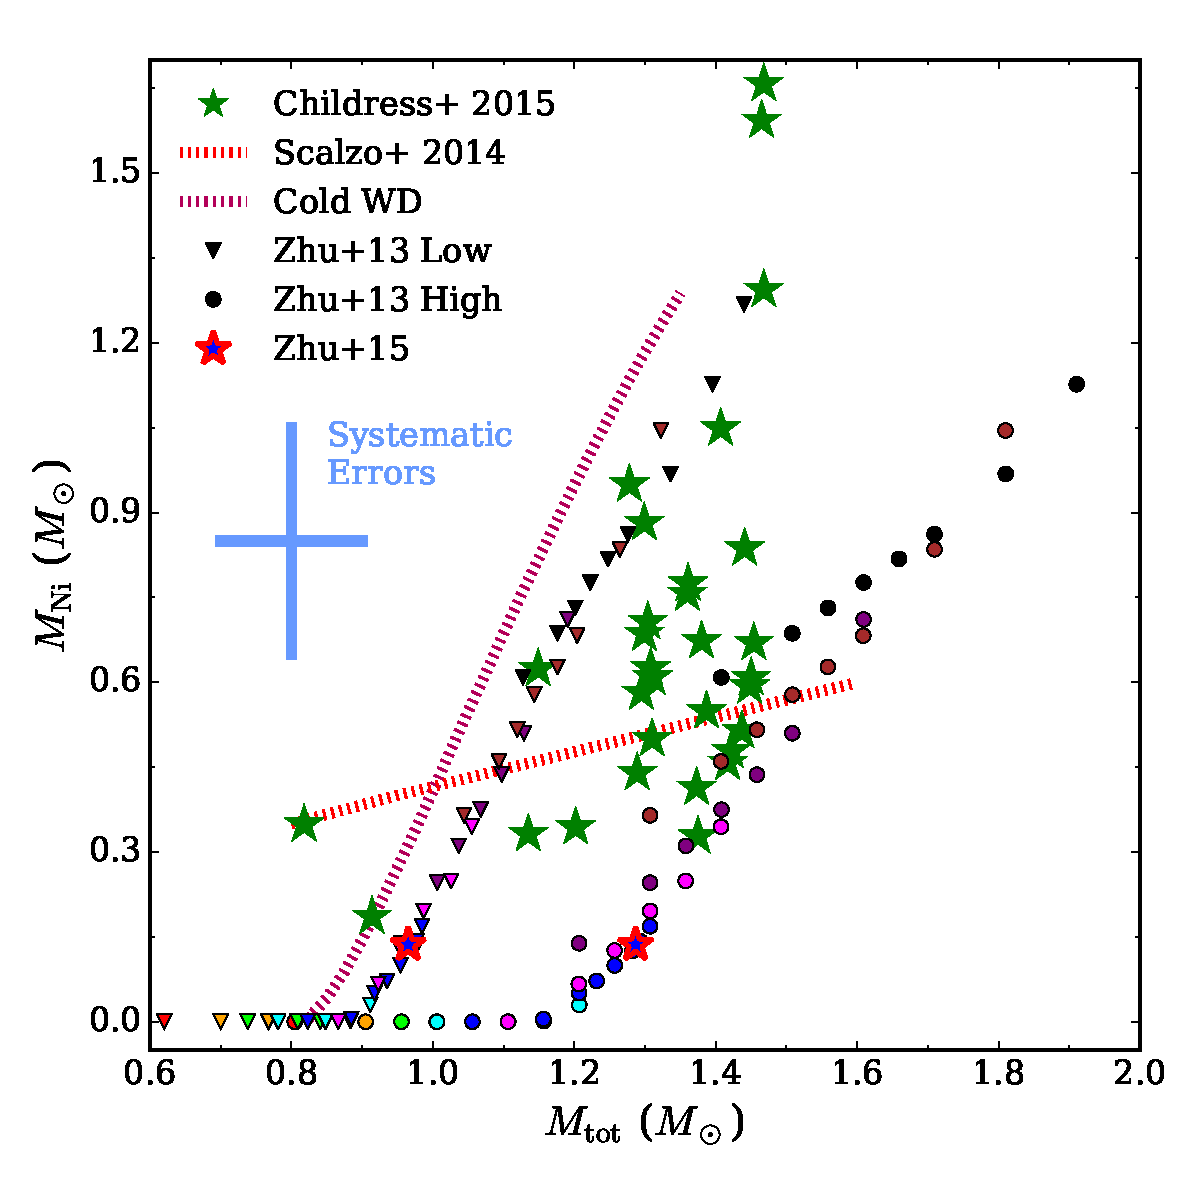
\includegraphics[angle=0,width=0.8\columnwidth]{conclusion/figures/c_MNi.pdf}
\caption{Relationships between total ejected mass \Mtot\ and synthesized \Ni\ mass \MNi\ for the merger remnants of Fig. \ref{fig:c2_pmevolution} if they were to (artificially) experience a pure detonation immediately after their estimated viscous spin-down.  \MNi\ is estimated by the mass of all remnant material with density $\rho>10^7\,\gcc$, $M(\rho>10^7)$.  \Mtot\ is estimated as the total mass of the remnant for the points, but we also extend lines leftward from each point to indicate how much of \Mtot\ is in the tenuous envelope.  Colors indicate accretor mass, as in Fig. \ref{fig:c2_constacc}.  Also plotted is the estimate for the \arepo\ MHD $0.625 - 0.65\,\Msun$ remnant (Ch. \ref{ch:ch4}; red-blue star).  All other features are as in Fig. \ref{fig:c5_mni}.}
\label{fig:c6_mcmce_mni}
\end{figure}

If powerful magnetic fields can indeed completely suppress convection, this will, at best, prevent any changes in the temperature and density structure of the WD once nuclear burning is lit.  If we assume this is the case, we can estimate the nucleosynthetic yields of our sub-\Mch\ merger remnants.  In Fig. \ref{fig:c6_mcmce_mni}, we show the total ejected mass \Mtot\ and synthesized \Ni\ mass \MNi\ of all the post-viscous remnants generated by the simple post-merger viscous evolution estimate in Sec. \ref{ssec:ch2_viscevo_possiblespindown} -- regardless of whether or not they are predicted to ignite nuclear burning -- if they were to detonate with no change to their structure.  \MNi\ is estimated by the mass of remnant material with density $\rho>10^7\,\gcc$.  It is not obvious how much of the tenuous post-viscous envelope should be included when estimating \Mtot, since some of it might have been ejected out to large distances.  We assume \Mtot\ is the total mass of the merger remnant for the points in Fig. \ref{fig:c6_mcmce_mni}, but from each point extend lines leftward by the mass of the envelope to bracket its inclusion.

Keeping in mind that our simple estimate tends to overestimate the amount of compression during viscous evolution, particularly for similar-mass mergers (Sec. \ref{sec:c2_postscript}), we see that only mergers with $\Mtot \gtrsim \Mch$ produce more than $\sim0.2\,\Msun$ of \Ni.  Since more realisitic simulations of viscous evolution predict less core compression, and not all remnants will ignite fusion, Fig. \ref{fig:c6_mcmce_mni} estimates the upper limit of \Ni\ produced by the sub-\Mch\ merger channel, and poses a challenge to its viability for producing normal SNe Ia.

\section{What are the Outcomes of CO WD Mergers?}

Considering the number of hurdles above, it appears that mergers of two CO WDs whose total mass is substantially below \Mch, including our fiducial $0.625 - 0.65\,\Msun$ merger, are unlikely to produce normal SNe Ia.  The more massive among them may ignite carbon burning, but these will probably become partly non-degenerate and expand before they achieve dynamical burning, eventually transforming their composition to O and Ne before cooling to become massive, highly-magnetized WDs.  Similar-mass super-\Mch\ WDs, on the other hand, may follow \citeal{vkercj10}'s evolutionary channel to ignite highly degenerate nuclear burning and eventually explode: mergers with accretors of $\gtrsim0.8\,\Msun$ create remnants that easily ignite nuclear burning during post-merger evolution and satisfy both the mass and central density constraints suggested by our simmering study.  Moreover, our rough estimate in Fig. \ref{fig:c6_mcmce_mni} shows their would produce \Ni\ masses consistent with normal SNe Ia.  This scenario for producing SNe Ia super-\Mch\ mergers is qualitatively different from the traditional one of slow accretion in eg. \cite{nomoi85} and \cite{yoonpr07}, though we cannot rule out the possibility of dissimilar-mass super-\Mch\ merger remnants avoiding off-center ignition and eventually cooling and compressing enough during thermal evolution \citep{shen+12} to start core pycnonuclear fusion.  Limiting explosion candidates to super-\Mch\ systems also leads to the same issue of rates that affects all other scenarios that require extremely massive WDs (Sec. \ref{ssec:c1_old_typeia}).

These super-\Mch\ binary systems, however, may have have already exploded in a violent merger (Sec. \ref{ssec:c1_new_typeia}), or shortly after coalescence due to accretion-heating from an $m = 1$ spiral mode \citep{kash+15}.  The minimum masses required for either is not well-known (see \citealt{dan+12, sato+16} for recent estimates for violent mergers), so it remains a task for future parameter-space merger studies to constrain them.
 
\section{Observational Avenues of Exploration}

Finally, we stress the potential of observational work in shedding light on this subject.  Recently revealed properties of the hot DQ population tantalizingly suggest they represent double CO WD merger remnants that did not explode.  Many of their fundamental properties, such as their masses and space density, remain poorly understood, but the Gaia mission will be able to provide parallaxes to help constrain these values \citep{dunl15thesis}.  Future observations will allow us to judge more confidently whether hot DQs are merger remnants.  If they are, the population's properties will serve as an observational check for the theoretical evolutionary scenarios in this work.

It may also be possible to spot merger remnants during their thermal evolution phase described in Sec. \ref{sec:c2_postscript}.  \cite{schw+16} consider the observable properties of their $1.5\,\Msun$ merger remnant, and calculate that it radiates on the order the Eddington luminosity for a $1.5\,\Msun$ star ($\sim10^5\,\Lsun$), and may also generate clouds of dust in its outermost layers, which will be launched as an optically thick wind.  This drives the remnant's photosphere out to $\sim10^{15}\,\mrm{cm}$, with a corresponding photospheric temperature of $\sim500\,\mrm{K}$, as well as possibly RCrB-like variablility of the remnant's luminosity.  \citep{schw+16} notes these features are similar to those of extreme AGB stars (eg. \citealt{blum+06}), and perhaps can be discovered using the same observational techniques.  Since sub-\Mch\ remnants have the same order of magnitude total energy as \Mch\ ones, their observed properties will be similar.

{\charles We have not yet modeled explosions of post-viscous merger remnants to determine if they photometrically and spectroscopically resemble SNe Ia.  Since they feature a sub-Keplerian disk through most of their evolution, and an extended envelope once they have ignited, they may look very different from typical SNe Ia.  See raskin's tamped explosions, kashyap's explosions, possibly talk about early UV flashes, Levanon's esetimates, etc.}

These new observational studies, alongside the theoretical and numerical discussed earlier, may clarify many of the outstanding questions posed throughout this thesis.  With luck, they will also lead to a clearer understanding of the fates of CO WD merger products, and SNe Ia.

%-resummarize all papers
%-don't say what we used to think

%-MRI growth rate in remnant?
%-simulation code does matter for post-merger evolution (hydrodynamic waves, magnetic fields)
%-They note that the luminosity of the nuclear burning zone is almost entirely carried away by neutrino losses (as the burning zone sits at the $\taucc = \taunu$ line), and so the remnant's source of luminosity is the heat from the merger and viscous evolution.

%\section{Does the \citeal{vkercj10} Channel Work?}

%Even if we assume runaways are vertical, the typical spun-down remnant still doesn't get to 1e7 gcc!

%%This result poses a problem for the \citeal{vkercj10} sub-\Mch\ merger channel.  \cite{shen+12} finds further compression could occur during the subsequent \textit{thermal} evolution of the remnant over $\gtrsim10^4\,\mrm{yr}$, which may allow more remnants to reach higher central density and enclose more mass within their cores.  Whether central burning could still begin is uncertain, however, since thermal diffusion and neutrino-driven cooling may favor off-center carbon ignition, or simply net cooling, even for those post-viscous remnants that are initially $\gtrsim5\times10^8\,\mrm{K}$ at their center.  Moreover, remnants, with radiation-dominated and highly magnetized carbon atmospheres, will likely drive strong outflows during their thermal evolution, further complicating predictions.  We note one advantage for delaying the explosion to during thermal evolution is the removal of the ``clutter'' of the $\gtrsim0.1\,\Msun$ hot envelope surrounding the core and extending out to $\gtrsim10^{11}\,\mrm{cm}$ \citep{shen+12}.  This imparts signatures onto the explosion not seen in ordinary SNe Ia, such as a double-peaked light curve from the shock cooling of the envelope, excess blue and UV emission prior to peak light, and a slow-decaying light curve near peak light \citep{frye+10,levasg15,pirom15}.  While \cite{shen+12}'s simulation suggests thermal evolution will do little to alter the overall structure of the envelope \citep{pirom15}, it does not account for mass loss due to winds.  These will significantly alter the size and structure of the envelope, perhaps mitigating its effects on any eventual explosion.  Meanwhile, material ejected from the remnant (both during its viscous and subsequent thermal phases) moving at the escape velocity will approach $\sim10^{17}\,\mrm{cm}$ after $\sim10^4\,\mrm{yr}$.  Interaction between this material and light from the supernova could explain \citep{shen+12, ji+13} observations of SN Ia-CSM interactions such as time-variable NaID lines (eg. \citealt{pata+07, simo+09}).

%% Magnetic coupling between the outflow and the remnant will aid in its spindown and possibly generate non-local heating through magnetic resistivity.

%Is the classic Mch DD channel even possible?

%-
%-





%\section{Observable Counterparts to Mergers}

%\section{The Evolution and Appearance of Quiescent Merger Remnants}

%% Shen+12 gives the escape velocity at 10^13 cm as 60 km/s.  Given 10^4 years of evolution, this wind could transport material to 10^18 cm, possibly explaining the variable sodium emission.

%\section{The Influence of Merger Remnants Properties on Potential Explosions}

%If sub-\Mch\ CO WD merger remnants indeed trigger thermonuclear detonations following post-merger viscous evolution, will these explosions resemble SNe Ia?  As noted in the introduction, SNe Ia observations and radiative transfer models for explosions are now sophisticated enough to distinguish fine details between different progenitors.  This question has been taken up by a number of theorists \citep{frye+10, shen+12}  Shen+12 conclusions!

%\cite{frye+10} and \cite{rask+14} do simulations

%\begin{itemize}
%	\item What are the mass loss rates of non-explosive mergers due to carbon dust superwind?  can we estimate?  could it possibly lead to Kepler's 0.6Msun oxygen WD? Shen+12 (Just under Eqn. 7) note that mass loss in radiation-dominated H/He-deficient envelopes is poor. %http://adsabs.harvard.edu/abs/2016Sci...352...67K
%	\item Near-eddington carbon burning star?  See Sec. 4 paragraph 1 of Shen+12.
%	\item Discussion with Marten: while we can't rule out further compression leading to nuclear burning during the thermal evolution phase, a combination of magnetically and Eddington-launched outflows will make the surroundings very messy - write more about this in SN Ia appearance stuff.
%	\item Importance of Ia-CSM stuff?  Shen+12 and Ji+13 (Sec. 2.2.3) have extensive sections on it.
%	\item Ji+13 has a mean magnetic field of 2e8 G; what does our simulation have?  They also (bottom of pg 7) give a quick estimate for magnetic lifetime.
%	\item What's the difference between a ring of material at $10^{13}$ cm and a continuous envelope that ends at the same radius?  Does one resemble Ia-CSM interaction, but the other lead to Fryer+10 or Piro+15 early time brightening?
%	\item Even super chandra DD systems will be much less dense than their WD binary progenitors - consequences for explosions?
%\end{itemize}



%\section{Avenues for Future Exploration}


%\subsection{Future Simulations of Mergers and Post-Merger Evolution}

%Do we need to simulate more merging WDs, especially using novel magnetohydrodynamic schemes?  Ch. STUFF suggests that the hydrodynamics up to coalescence and overall remnant properties do not substantively change when transitioning from simulating with a traditional variant of SPH to doing so with a modern moving mesh code, and getting the initial conditions (eg. synchronization, accurate tidal bulges for the onset of mass transfer) right is likely to be more important.  We await results from the the Eulerian grid WD merger simulations of \citep{katz+16} for further confirmation.

%What does require further work is the magnetic evolution during the merger, as well as the early phase of post-merger evolution and further magnetic field growth following coalescence.  The former has been insufficiently investigated with the latest generation of MHD codes, which may end up predicting very different field configurations (and possibly energies) than our exploration of the problem with \arepo.  The latter, however, is not only also poorly explored (only one group has conducted a full MHD simulation!) but essential to better understanding post-merger evolution.  This regime is particularly challenging for codes, since it requires the code minimize numerical hydrodynamic and magnetic viscosity (traditionally problematic for SPH codes) while maintaining conservative quantities -- particularly angular momentum -- over hundreds of dynamical times (traditionally difficult for grid codes).  Moreover, the problem is stiff, since evolution occurs both on a dynamical (with spiral waves) and viscous timescale, and thus quite computationally intensive.  We note the recent introduction of two codes: duffel's and hopkins', that could potentially bridge the gap.

%Arepo MHD doesn't do a good job of conserving angular momentum - balance plot shows it spurious gains it.  May be due to divergence cleaning (hopkins 16)


%Simulations of detonations within violent mergers (eg. \ref{pakm+10, bull+16, krom+16}) or mergers shortly after coalescence \citep{rask+14,vros+15}, do not reproduce the light curves and spectra of SNe Ia.  

%OUR REMNANTS AREN'T RADIATION DOMINATED.  Prad/Pion \propto T^3/\rho \propto \rho in adiabatic envelopes; we're in general much colder for any given density than Shen+12, so in fact we don't have radiation dominated envelopes, but we still have extended ones!

%Shen+16 is important, since nuclear burning energy doesn't get to exterior before 1e4 years are up, so non-burning remnants will look similar!

%It may also be possible to spot merger remnants during their thermal evolution phase described in Sec. \ref{sec:c2_postscript}.  \cite{schw+16} consider in depth the observable properties of their $\1.5\,\Msun$ merger remnant undergoing carbon and neon burning.  They note that the luminosity of the nuclear burning zone is almost entirely carried away by neutrino losses (as the burning zone sits at the $\taucc = \taunu$ line), and so the remnant's source of luminosity is the heat from the merger and viscous evolution.  Since sub-\Mch\ remnants have the same order of magnitude total energy as \Mch\ ones, their observed properties will be similar.  \cite{schw+16} find that, with an envelope and a radiation-dominated hot atmosphere of $10^{12}-10^{13}\,\mrm{cm}$, the remnant initially radiates of order the Eddington luminosity for a $1.5\,\Msun$ star ($\sim10^5\,\Lsun$) and has a photospheric temperature ranging from $4000 - 10^5\,\mrm{K}$.  The remnant may also generate clouds of dust in their outermost layers, which will then be launched as an optically thick wind, driving the remnant's photosphere out to $\sim10^{15}\,\mrm{cm}$, with corresponding photospheric temperatures of $\sim500\,\mrm{K}$, and lead to RCrB-like variablility in the remnant's luminosity.  \citep{schw+16} notes these features are similar to those of extreme AGB stars (eg. \citealt{blum+06}).

%krom+16 http://adsabs.harvard.edu/doi/10.1093/mnras/stw962
%bull+16 http://adsabs.harvard.edu/abs/2016MNRAS.455.1060B
%vros+15 http://adsabs.harvard.edu/abs/2015arXiv151004286V
%papi+15 http://adsabs.harvard.edu/abs/2015MNRAS.449..942P
%pirom15 http://adsabs.harvard.edu/abs/2015arXiv151203442P



%% This adds a line for the Bibliography in the Table of Contents.
\addcontentsline{toc}{chapter}{Bibliography}
%% *** Set the bibliography style. ***
%% (change according to your preference/requirements)
\bibliographystyle{apj}
%% *** Set the bibliography file. ***
%% ("thesis.bib" by default; change as needed)
\bibliography{AutoBibliography}

%% *** NOTE ***
%% If you don't use bibliography files, comment out the previous line
%% and use \begin{thebibliography}...\end{thebibliography}.  (In that
%% case, you should probably put the bibliography in a separate file and
%% `\include' or `\input' it here).

\end{document}

%citation{frye+10}{2010ApJ...725..296F}	%Fryer double degenerate light curves.
%citation{rask+14}{2014ApJ...788...75R}	%Cody's tamped explosion models.
%citation{bigness+15}{2015ApJ...788..BIG}


%citation{badem12}{2012ApJ...749L..11B} %Badenes and Moaz's paper on galactic WD merger rate from SDSS
%citation{saioj00}{2000MNRAS.313..671S}	%saio and jeffrey He - He merger
%citation{justph11}{2011MNRAS.410..984J} %stephen's sdO star from He - He merger
%citation{webb84}{1984ApJ...277..355W} %Webbink was one of the first to suggest He - CO -> RCB
%citation{saioj02}{2002MNRAS.333..121S}	%saio and jeffrey He - CO merger
%citation{clay+07}{2007ApJ...662.1220C} %Clayton's 18O/16O abundance and mergers making RCB stars
%citation{clay13}{2013ASPC..469..133C} %Clayton's review on mergers making rCB stars
%citation{segrcm97}{1997ApJ...481..355S} %SPH simulation
%citation{garc+12}{2012ApJ...749...25G} %garcia-berro et al. on white dwarf mergers generating strong magnetic fields
%citation{kule+13}{2013MNRAS.431.2778K} %kulebi's disk/remnant coupling model, which attempts to predict final HFMWD spins
%citation{dunlc15}{2015ASPC..493..547D} %bart and chris's work published in conference proceeding
%citation{saion85}{1985A&A...150L..21S} % edge-lit ignition
%citation{abdi+10}{2010PhRvD..81d4012A} %GR simulation of AIC
%citation{maozmn14}{2014ARA&A..52..107M} %Maoz's review paper
%citation{hill+13}{2013FrPhy...8..116H}	%hillebrandt's recent SN Ia review paper


%citation{dist10}{2010ApJ...719..474D}
%citation{loreig09}{2009A&A...500.1193L}
%citation{mann+05}{2005A&A...433..807M}
%citation{maozsg10}{2010ApJ...722.1879M}
%citation{menn+10}{2010ASPC..435...33M}
%citation{mona05}{2005RPPh...68.1703M}
%citation{pakm+10}{2010Natur.463...61P}
%citation{pakm+11}{2011A&A...528A.117P}
%citation{paxt+11}{2011ApJS..192....3P}
%citation{ries+98}{1998AJ....116.1009R}
%citation{vkercj10}{2010ApJ...722L.157V}
%citation{wadssq04}{2004NewA....9..137W}
%citation{perl+99}{1999ApJ...517..565P}
%citation{ruitbf09}{2009ApJ...699.2026R}
%citation{sim+10}{2010ApJ...714L..52S}
%citation{dan+11}{2011ApJ...737...89D}
%citation{yoonpr07}{2007MNRAS.380..933Y}
%citation{guerig04}{2004A&A...413..257G}
%citation{timms00}{2000ApJS..126..501T}
%citation{mona92}{1992ARA&A..30..543M}
%citation{segrcm97}{1997ApJ...481..355S}
%citation{marsns04}{2004MNRAS.350..113M}
%citation{marsns04}{2004MNRAS.350..113M}
%citation{mars11}{2011CQGra..28i4019M}
%citation{eggl83}{1983ApJ...268..368E}
%citation{geroh89}{1989ApJS...70..661G}
%citation{maoz10}{2010AIPC.1314..223M}
%citation{ruit+11}{2011MNRAS.417..408R}
%citation{nomoi85}{1985ApJ...297..531N}
%citation{guil+10}{2010ApJ...709L..64G}
%citation{justph11}{2011MNRAS.410..984J}
%citation{woosk11}{2011ApJ...734...38W}
%citation{fink+10}{2010A&A...514A..53F}
%citation{saion98}{1998ApJ...500..388S}
%citation{kube+10}{2010A&A...524A..36K}
%citation{dan+12}{2012MNRAS.422.2417D}
%citation{rask+12}{2012ApJ...746...62R}
%citation{benz+90}{1990ApJ...348..647B}
%citation{krom+10}{2010ApJ...719.1067K}
%citation{dsou+06}{2006ApJ...643..381D}
%citation{lairs94}{1994ApJ...437..742L}
%citation{uryue98}{1998ApJS..118..563U}
%citation{fulll12}{2012MNRAS.421..426F}
%citation{piro11}{2011ApJ...740L..53P}
%citation{shen+12}{2012ApJ...748...35S}
%citation{gera+07}{2007ApJ...661..995G}
%citation{stei+10}{2010ApJ...716L.146S}
%citation{brow+11}{2011ApJ...737L..23B}
%citation{seit+09}{2009ApJ...696..515S}
%citation{schw+12}{2012MNRAS.427..190S}
%citation{balbh91}{1991ApJ...376..214B}
%citation{spru02}{2002A&A...381..923S}
%citation{shaks73}{1973A&A....24..337S}
%citation{maed+10}{2010ApJ...708.1703M}
%citation{frye+10}{2010ApJ...725..296F}
%citation{vker13}{2013RSPTA.37120236V}
%citation{haye+06}{2006ApJS..165..188H}
%citation{tremb09}{2009ApJ...696.1755T}
%citation{spri10a}{2010ARA&A..48..391S} %SPH review
%citation{gilfb10}{2010Natur.463..924G}
%citation{rappds94}{1994ApJ...426..692R}
%citation{bloo+12}{2012ApJ...744L..17B}
%citation{bars+95}{1995MNRAS.277..971B}  % RE 
%citation{hama97}{1997IAUS..180...91H} % [WR] wind mass loss rates
%citation{saion85}{1985A&A...150L..21S} % edge-lit ignition
%citation{woos+09}{2009ApJ...704..255W} % deflagration, density effects
%citation{woos+11}{2011ApJ...734...37W} % ...
%citation{aspd+11}{2011ApJ...738...94A} % rising deflagration bubbles
%citation{maed+10a}{2010ApJ...708.1703M} % nebular, offset dense stuff
%citation{maed+10b}{2010Natur.466...82M} % idem
%citation{taub+09}{2011MNRAS.412.2735T} % slow-moving superchandrasekhar
%citation{spri10b}{2010MNRAS.401..791S} % AREPO
%citation{duffm11}{2011ApJS..197...15D} % TESS
%citation{shig+92}{1992ApJ...386L..13S}  % sub-Ch -> right nucleosyn/energetics
%citation{mazumw77}{1977ApJ...213..518M}
%citation{hernk89}{1989ApJS...70..419H}	%Gasoline's kernel
%citation{seitcr11}{2011MNRAS.414.2709S}

%citation{ji+13}{2013ApJ...773..136J}
%citation{dan+14}{2014MNRAS.438...14D}
%citation{rask+13}{2013arXiv1312.3649R}	%Part 2 of Cody's merger work
%citation{moll+14}{2014ApJ...785..105M}	%Part 1 of Cody's merger work
%citation{pakm+13}{2013ApJ...770L...8P} %ruediger's helium paper
%citation{zhu+13}{2013ApJ...767..164Z} %my sph paper
%citation{pakm+12}{2012ApJ...747L..10P} $ruediger's sph paper
%citation{dehna12}{2012MNRAS.425.1068D}
%citation{voge+12}{2012MNRAS.425.3024V} %arepo explicit refinement for maintaining fixed mass
%citation{nels+13}{2013MNRAS.429.3353N} %Gas accretion in cosmo sims
%citation{pakmv13}{2013MNRAS.432..176P}
%citation{marips14}{2014MNRAS.437.1750M} %Galaxy formation in cosmo sims
%citation{hayw+13}{2013arXiv1309.2942H}	%Galaxy mergers in Arepo
%citation{spri05}{2005MNRAS.364.1105S} %gadget2
%citation{ager+07}{2007MNRAS.380..963A} %SPH instability failure paper
%citation{hubbfg13}{2013MNRAS.432..711H}
%citation{baues12}{2012MNRAS.423.2558B}	%SPH turblence capture
%citation{pric08}{2008JCoPh.22710040P}	%artificial conductivity to improve SPH mixing/instability
%citation{hopk13}{2013MNRAS.428.2840H}	%pressure-entropy formulation of SPH
%citation{lanz10}{2010MNRAS.408.2336L} %switching up the EOS improves spiral arm capture
%NOT SURE IF WE WANT THIS {lanz10a}{2010MNRAS.408.1551L}

%citation{lanz03}{2003A&A...403..593L}	%effect of varying viscosity on spiral wave formation
%citation{lanzb97}{1997MNRAS.284..957L}	%3D SPH spiral wave sims
%citation{savopl94}{1994MNRAS.268...13S}	%spiral waves in disks.
%citation{sawamh86}{1986MNRAS.219...75S}	%spiral waves in disks.
%citation{dval+06}{2006MNRAS.370..529D}	%planet migration code comparison
%citation{kleyn12}{2012ARA&A..50..211K}	%planet migration review
%citation{balb03}{2003ARA&A..41..555B}	%spiral wave review
%citation{yukabm97}{1997MNRAS.292..321Y} %3D SPH spiral wave sims; intro describes the issue of artificial viscosity
%citation{burk+13}{2013MNRAS.433..332B}	%tides in WD binaries
%citation{shaks73}{1973A&A....24..337S} %Shakura and Sunyaev 1973 paper including alpha viscosity
%citation{mitc+09}{2009MNRAS.395..180M}	%SPH/Eulerian code comparison for galaxy cluster formation
%citation{tracsp07}{2007MNRAS.377..997T}	%SPH/Eulerian code comparison for stellar collisions
%citation{maed+13}{2013A&A...553A...1M}	%general stability criterion for rotating stars
%citation{justph11}{2011MNRAS.410..984J}	%stephen justham's sdO paper
%citation{webb84}{1984ApJ...277..355W} %webbink's classic paper
%citation{clay+07}{2007ApJ...662.1220C}	%clayton's 2007 paper on RCB abundances
%citation{jeffks11}{2011MNRAS.414.3599J} %jeffrey's 2011 paper on RCB abundances  NOT CURRENTLY USED
%citation{hill+13}{2013FrPhy...8..116H}	%hillebrandt's recent SN Ia review paper
%citation{loke+10}{2010JPhCS.256a2026L}	%SciNet paper
%citation{ross14}{2014arXiv1406.4224R} %rosswog's SPH review
